% !TEX root = ../main.tex
\section{Experiments}
\label{sec:experiments}

This section evaluates CLoMC-UWR with the evaluation suite in
Section~\ref{sec:evaluation-suite} through three settings. The first examines
whether CLoMC-UWR outperforms an Optimization-Based Planner as
operational pressure increases and how sensitive it is to model choice. The
second isolates how Validation, Memory, and Runtime Replanning address their
respective decision risks, while the third tests whether validated
demonstrations can specialize a compact planner with lower planning overhead.
The following subsections specify the experimental setup and then report the
end-to-end, ablation, and fine-tuned planner evaluations.

\subsection{Experimental Setup}

\subsubsection{End-to-End Setting}
We fix Gemini~3.1~Pro for Vision Analysis and use ChatGPT~5.5,
Gemini~3.1~Pro, Claude~Opus~4.7, or DeepSeek~V4~Pro in Mission Planning,
Validation, and Runtime Replanning. Fixing Vision Analysis keeps the
structured fire situation consistent, so differences among the four downstream
foundation-model configurations reflect the downstream decision process.

The Optimization-Based Planner is implemented with the CP-SAT solver in Google
OR-Tools. It shares the Vision Analysis output, UAV operational states, mission constraints,
and action space with CLoMC-UWR, and re-optimizes the remaining
task chains from the updated operational state after each runtime perturbation.
Its downstream decision process does not use an LLM, Validation, or Memory. The
baseline and four foundation-model configurations use the same 80 episodes---20
at each difficulty level---and the same execution and scoring procedure.

\subsubsection{Ablation Setting}
Using the DeepSeek~V4~Pro configuration, we compare CLoMC-UWR with w/o
Validation, w/o Memory, and w/o Runtime Replanning. These variants respectively
remove Validation, disable retrieval from Memory, and retain the initial plan
after runtime perturbations. All other models, prompts, and execution settings
remain unchanged, and all four configurations use the same 80 episodes, with 20
at each difficulty level.
Because simple and normal episodes contain no runtime perturbations, Runtime
Replanning remains inactive; the w/o Runtime Replanning variant therefore
introduces no other execution difference at these levels.

\subsubsection{Fine-Tuning Data and Training}
We construct 2,000 mission-planning demonstrations using CLoMC-UWR
with Gemini~3.1~Pro as the teacher planner from mission situations disjoint from
the 80 evaluation episodes. Each demonstration maps $(\mathcal{Z},U,C)$ to $P$, pairing
the task zones, UAV operational states, and mission constraints with the final multi-UAV
plan accepted by Validation. These validated demonstrations specialize
Qwen3-8B for the planning mapping in Section~\ref{sec:system-design}. We use a
90\%/10\%
training/validation split and 4-bit quantized low-rank adaptation with a maximum
sequence length of 6,144 tokens, three epochs, an effective batch size of 16,
and a learning rate of $5\times10^{-5}$. Fine-tuning uses one NVIDIA GeForce
RTX~4090, 16 Intel Xeon Gold~6430 vCPUs, and 120~GB of system memory.

\subsubsection{Planner Evaluation Protocol}
We evaluate the original and fine-tuned Qwen3-8B by replacing only the planner
used by Mission Planning. Vision Analysis and Validation retain
Gemini~3.1~Pro, while all non-LLM components remain unchanged. Both
configurations use the same 40 simple and normal episodes---20 at each
level---from the first setting. Because these episodes
contain no runtime perturbations, the experiment neither invokes Runtime
Replanning nor assesses event stability, thereby isolating planner fine-tuning.

\subsection{End-to-End Evaluation}

Table~\ref{tab:main-results} reports the end-to-end results, while
Figures~\ref{fig:model-total-score} and~\ref{fig:model-performance-radar}
summarize the overall scores and mission-level profiles.

\begin{figure}[!t]
    \centering
    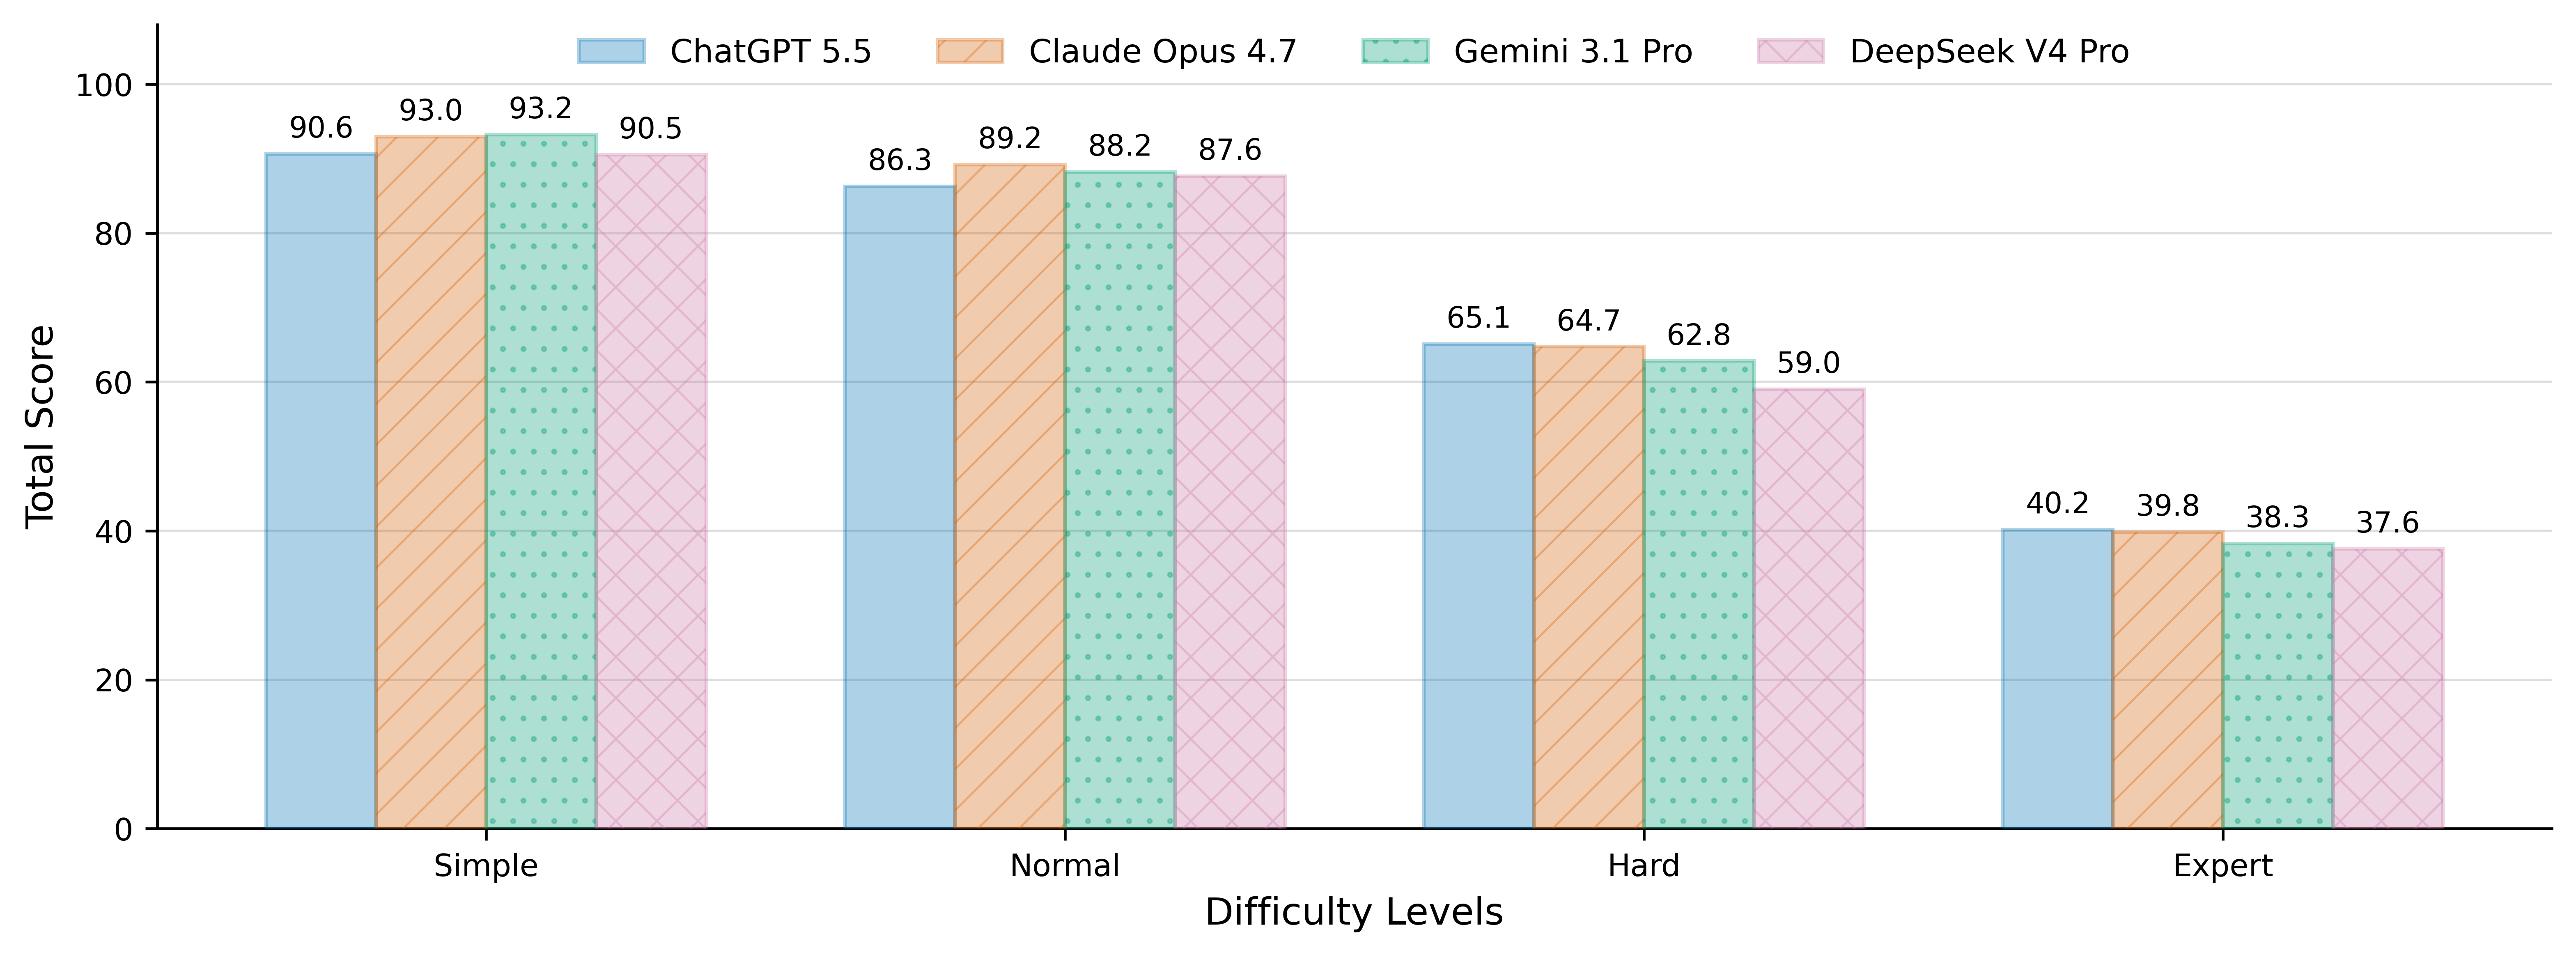
\includegraphics[width=\columnwidth]{figures/foundation-model-overall-scores.png}
    \caption{Overall scores of the Optimization-Based Planner and four
    foundation-model configurations across episode difficulty levels.}
    \label{fig:model-total-score}
\end{figure}

\begin{table*}[!t]
    \centering
    \caption{End-to-end results for the Optimization-Based Planner and the
    proposed framework across episode difficulty levels. Optimization-Based
    denotes the Optimization-Based Planner, while each model name denotes the
    corresponding downstream foundation-model configuration of the proposed
    framework.
    $S$ is the overall score, and the remaining columns report normalized mission-level scores in
    $[0,100]$ (higher is better). Event stability is not applicable to the
    simple and normal settings and is denoted by ``--''. The highest observed
    value for each metric at every difficulty level is shown in bold when it is
    unique; these highlights describe the evaluated configurations rather than
    a general ranking of foundation models.}
    \label{tab:main-results}
    \footnotesize
    \setlength{\tabcolsep}{1.5pt}
    \renewcommand{\arraystretch}{1.12}
    \begin{tabular*}{\textwidth}{@{\extracolsep{\fill}}llcrrrrrr@{}}
        \toprule
        \multirow{2}{*}{\textbf{Difficulty}}
        & \multirow{2}{*}{\textbf{Configuration}}
        & \multirow{2}{*}{\textbf{$S$}}
        & \multicolumn{6}{c}{\textbf{Mission-level score}} \\
        \cmidrule(l){4-9}
        & &
        & \textbf{Completion}
        & \textbf{Response}
        & \textbf{Time}
        & \makecell{\textbf{Event}\\\textbf{stability}}
        & \makecell{\textbf{Resource}\\\textbf{pressure}}
        & \textbf{Coordination} \\
        \midrule

        Simple & Optimization-Based
        & 92.59 & 100.00 & \textbf{92.34} & 88.94
        & -- & \textbf{85.64} & 82.31 \\
        & ChatGPT~5.5
        & 90.63 & 100.00 & 89.18 & 78.99
        & -- & 81.20 & 79.54 \\
        & Gemini~3.1~Pro
        & \textbf{93.23} & 100.00 & 88.78 & \textbf{91.06} & -- & 84.45 & 80.71 \\
        & Claude~Opus~4.7
        & 92.97 & 100.00 & 91.44 & 86.62 & -- & 82.18 & \textbf{83.96} \\
        & DeepSeek~V4~Pro
        & 90.54 & 100.00 & 87.66 & 78.90 & -- & 83.05 & 80.04 \\
        \addlinespace

        Normal & Optimization-Based
        & 88.72 & 100.00 & 89.07 & \textbf{72.71}
        & -- & \textbf{87.05} & 77.74 \\
        & ChatGPT~5.5
        & 86.28 & 100.00 & 93.82 & 66.27
        & -- & 77.64 & 73.19 \\
        & Gemini~3.1~Pro
        & 88.23 & 100.00 & 94.10 & 71.50 & -- & 86.68 & 71.72 \\
        & Claude~Opus~4.7
        & \textbf{89.18} & 100.00 & \textbf{96.09} & 68.24 & -- & 84.54 & \textbf{78.12} \\
        & DeepSeek~V4~Pro
        & 87.63 & 100.00 & 91.36 & 71.74 & -- & 83.95 & 75.13 \\
        \addlinespace

        Hard & Optimization-Based
        & 49.77 & 96.40 & 78.32 & 26.94
        & 20.75 & 54.86 & 52.14 \\
        & ChatGPT~5.5
        & \textbf{65.09} & 100.00 & \textbf{94.97} & \textbf{41.22}
        & \textbf{42.25} & \textbf{63.19} & \textbf{67.24} \\
        & Gemini~3.1~Pro
        & 62.81 & 100.00 & 92.58 & 39.60 & 33.75 & 59.10 & 60.65 \\
        & Claude~Opus~4.7
        & 64.74 & 99.86 & 94.22 & 35.28 & 40.50 & 62.15 & 65.88 \\
        & DeepSeek~V4~Pro
        & 59.03 & 98.57 & 83.90 & 30.76 & 34.75 & 61.36 & 59.07 \\
        \addlinespace

        Expert & Optimization-Based
        & 21.53 & 78.27 & 42.13 & 1.93
        & 0.00 & 42.07 & 39.87 \\
        & ChatGPT~5.5
        & \textbf{40.15} & \textbf{93.24} & \textbf{67.01} & \textbf{13.23}
        & \textbf{2.67} & \textbf{60.15} & \textbf{61.25} \\
        & Gemini~3.1~Pro
        & 38.28 & 90.09 & 61.30 & 12.02 & 0.00 & 58.72 & 55.82 \\
        & Claude~Opus~4.7
        & 39.81 & 92.43 & 65.55 & 9.13 & 0.00 & 58.99 & 60.11 \\
        & DeepSeek~V4~Pro
        & 37.55 & 90.95 & 61.09 & 3.54 & 0.00 & 53.43 & 54.43 \\
        \bottomrule
    \end{tabular*}
\end{table*}


In the simple and normal settings, where no runtime perturbations occur, all
evaluated methods achieve complete task coverage. The Optimization-Based
Planner obtains overall scores of 92.59 and 88.72, respectively, which lie
within the corresponding ranges of the four foundation-model configurations
(90.54--93.23 and 86.28--89.18), confirming that it remains competitive under
lower operational pressure.

Once runtime perturbations are introduced, the difference between the two
decision approaches becomes more pronounced: the Optimization-Based Planner
scores 49.77 and 21.53 in the hard and expert settings, respectively 9.26 and
16.02 points below the lowest-scoring foundation-model configuration. Its expert
completion score is 78.27, compared with 90.09--93.24 for the four
configurations. Because its event stability score of 0 overlaps their 0--2.67
range, the advantage of CLoMC-UWR also reflects task completion
and the other execution-quality metrics.

\begin{figure}[!htbp]
    \centering
    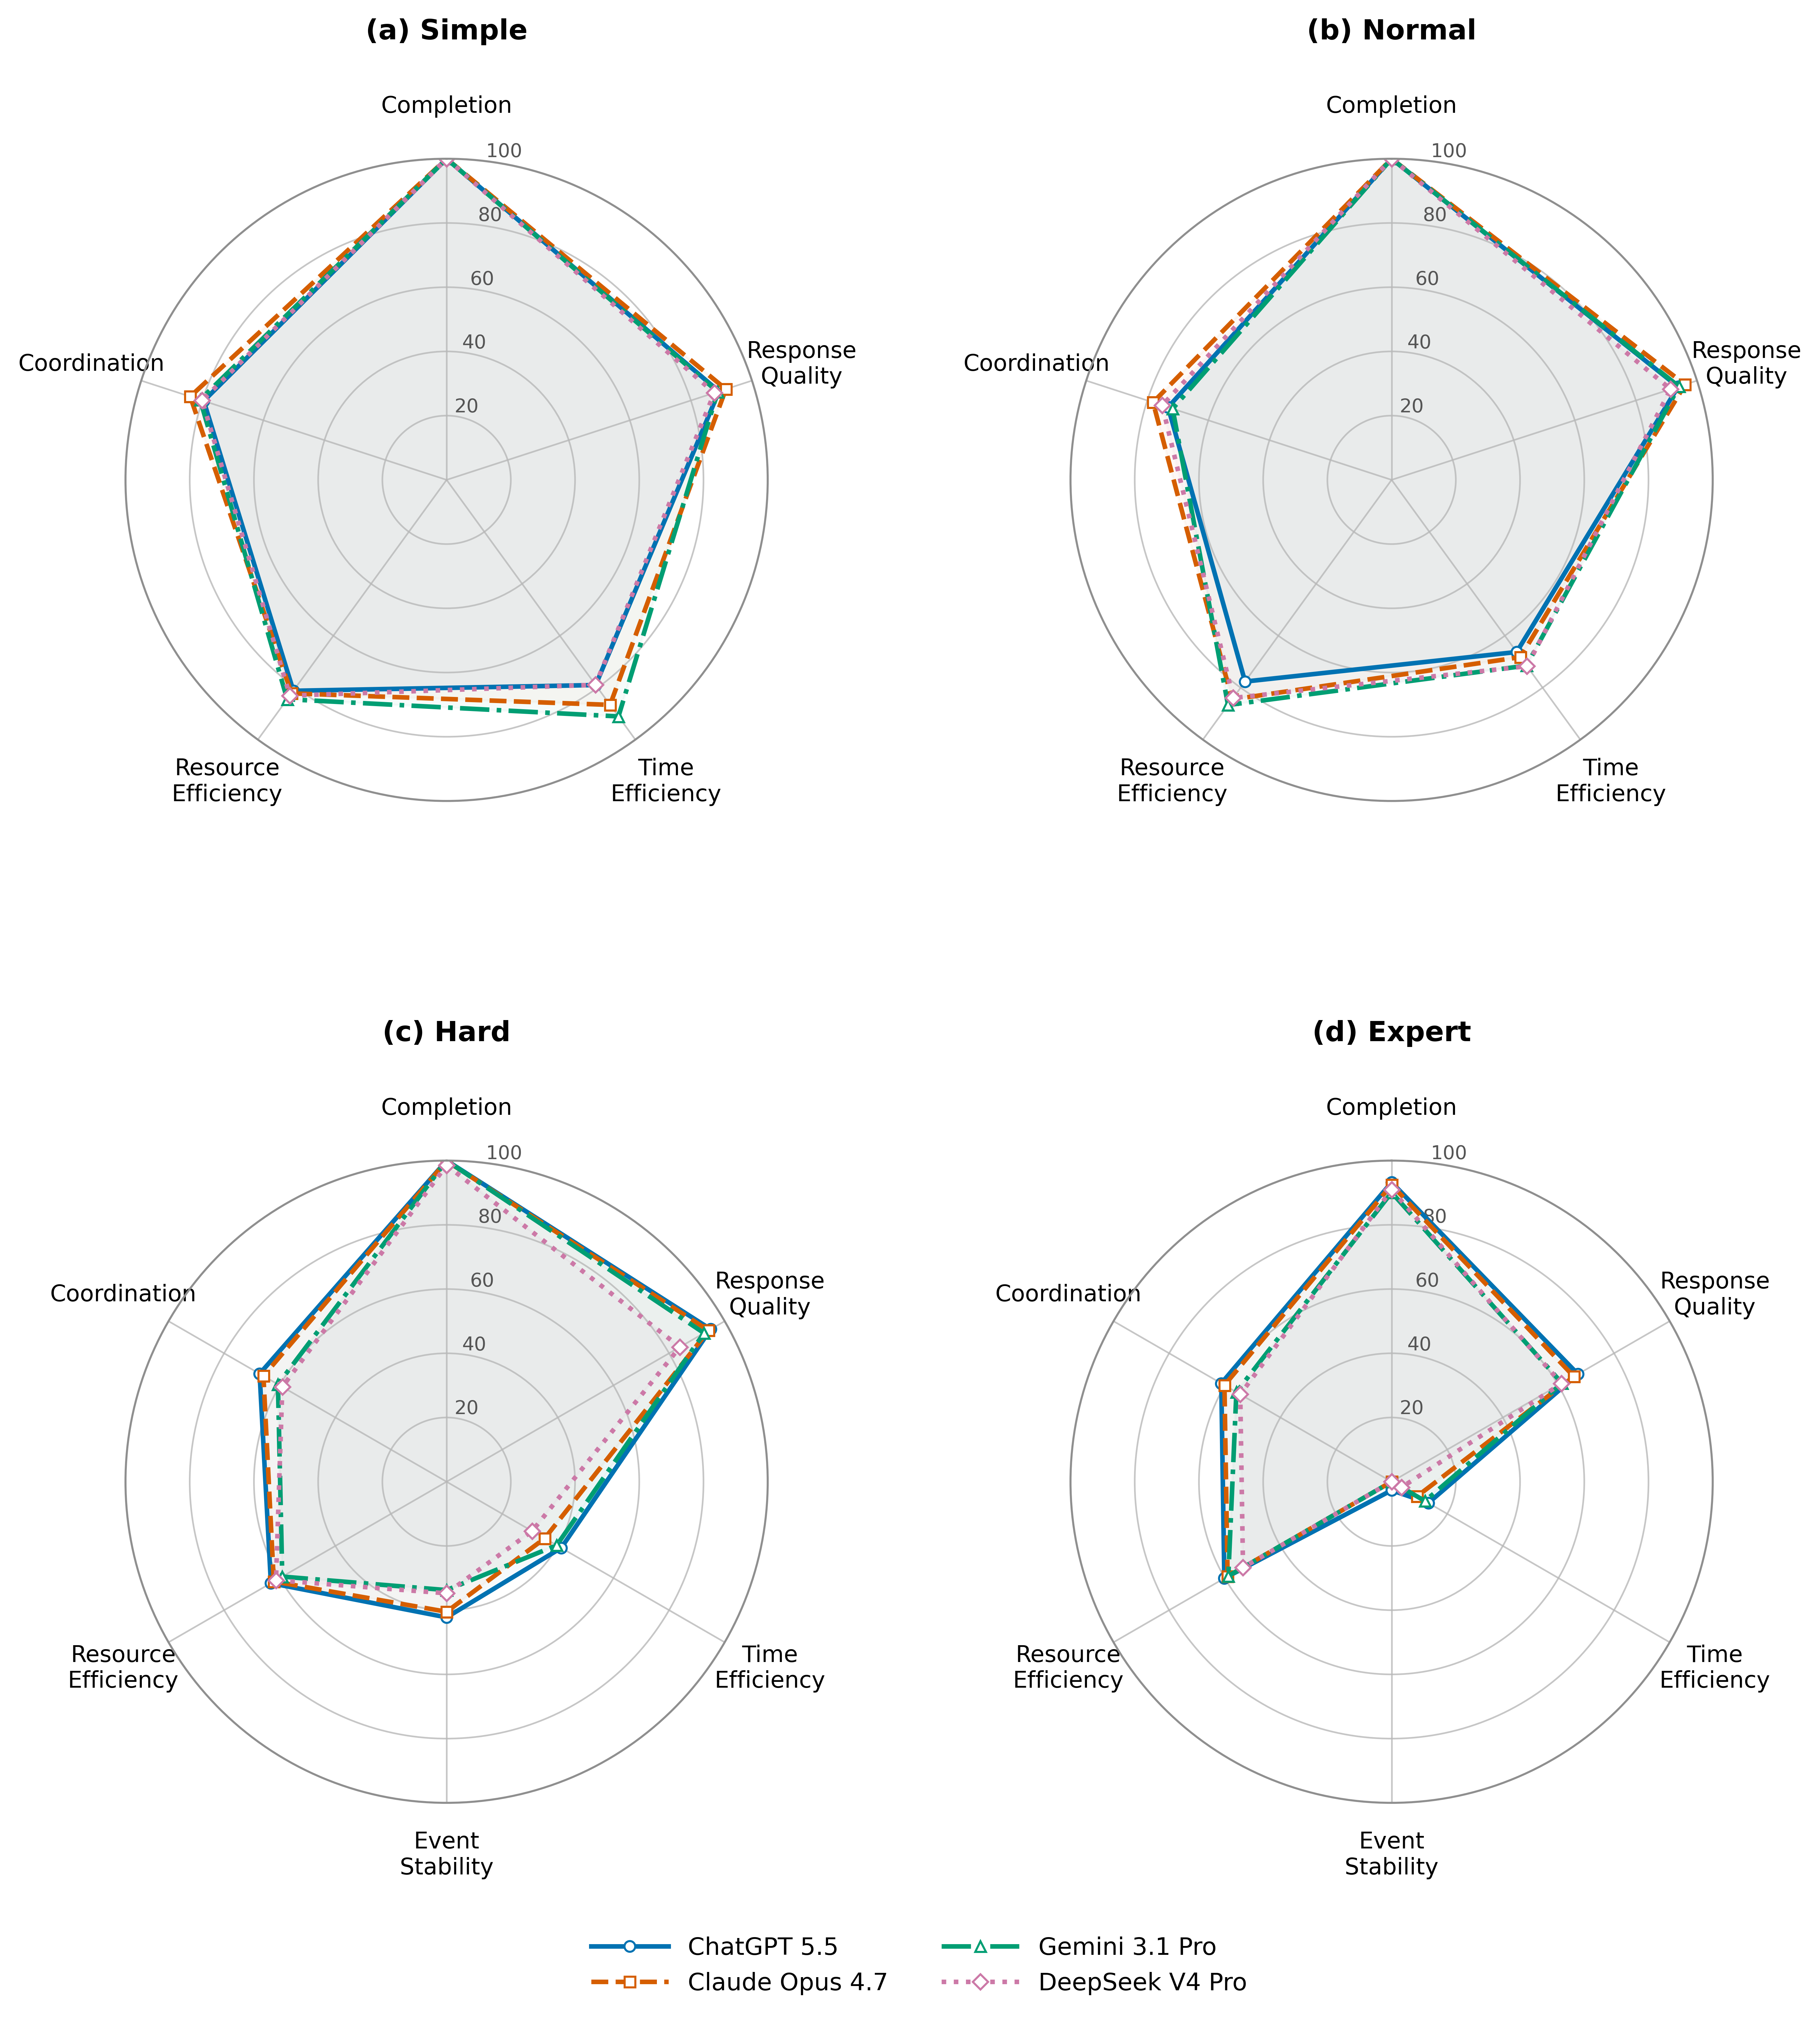
\includegraphics[width=0.95\columnwidth]{figures/foundation-model-performance-radar.png}
    \caption{Mission-level performance profiles of the Optimization-Based
    Planner and four foundation-model configurations at each difficulty level.
    Larger radial values indicate better performance.}
    \label{fig:model-performance-radar}
\end{figure}

Among the four foundation-model configurations, Gemini~3.1~Pro obtains the
highest overall score in the simple setting, Claude~Opus~4.7 in the normal
setting, and ChatGPT~5.5 in the hard and expert settings. Because this ordering
changes with difficulty, the results do not yield a single model ranking. All
four configurations maintain high basic task completion in the hard and expert
episodes, but their mission time scores fall to 3.54--13.23 and their event
stability scores to 0--2.67 under expert conditions. Model choice thus
affects the downstream decision process, but changing the foundation model
alone does not prevent the common degradation as operational pressure
increases.

Taken together, the Optimization-Based Planner remains competitive in the
simple and normal episodes, where no runtime perturbations occur. Under the
higher operational pressure of the hard and expert episodes, CLoMC-UWR
maintains higher basic task completion and execution quality across
all four downstream foundation-model configurations. The common decline in
mission time and event stability under expert conditions nevertheless leaves
clear headroom for more robust replanning and time-aware resource allocation.

\subsection{Ablation Studies}

Table~\ref{tab:ablation-results} reports the ablation results with
DeepSeek~V4~Pro fixed as the foundation model. Removing Validation causes a
modest but consistent reduction across all four difficulty levels, with drops
of 2.16, 2.33, 3.81, and 2.05 points from simple to expert. The limited change
in average mission score does not imply that the module remains inactive: the
validation loop is triggered 5, 5, 4, and 6 times in the simple, normal, hard,
and expert settings, respectively. These interventions suggest that Validation
primarily serves as an occasional reliability safeguard against invalid or
tactically implausible plans rather than as a continuous source of score
improvement.

\begin{table}[!htbp]
    \centering
    \caption{Ablation results with DeepSeek~V4~Pro as the foundation model.
    Values report the mean overall score $S$ over 20 episodes at each
    difficulty level. The best result in each column is shown in bold.}
    \label{tab:ablation-results}
    \small
    \setlength{\tabcolsep}{7pt}
    \renewcommand{\arraystretch}{1.15}
    \begin{tabular}{@{}lcccc@{}}
        \toprule
        \multirow{2}{*}{\textbf{Configuration}}
        & \multicolumn{4}{c}{\textbf{Overall score $S$}} \\
        \cmidrule(l){2-5}
        & \textbf{Simple} & \textbf{Normal} & \textbf{Hard} & \textbf{Expert} \\
        \midrule
        Full
        & \textbf{90.54} & 87.63 & \textbf{59.03} & \textbf{37.55} \\
        w/o Validation
        & 88.38 & 85.30 & 55.22 & 35.50 \\
        w/o Memory
        & 88.57 & 86.94 & 49.35 & 22.10 \\
        w/o Runtime Replanning
        & 90.33 & \textbf{88.14} & 35.86 & 12.98 \\
        \bottomrule
    \end{tabular}
\end{table}


Figure~\ref{fig:ablation-score-delta} visualizes the score change of each
ablated variant relative to CLoMC-UWR.

\begin{figure}[!t]
    \centering
    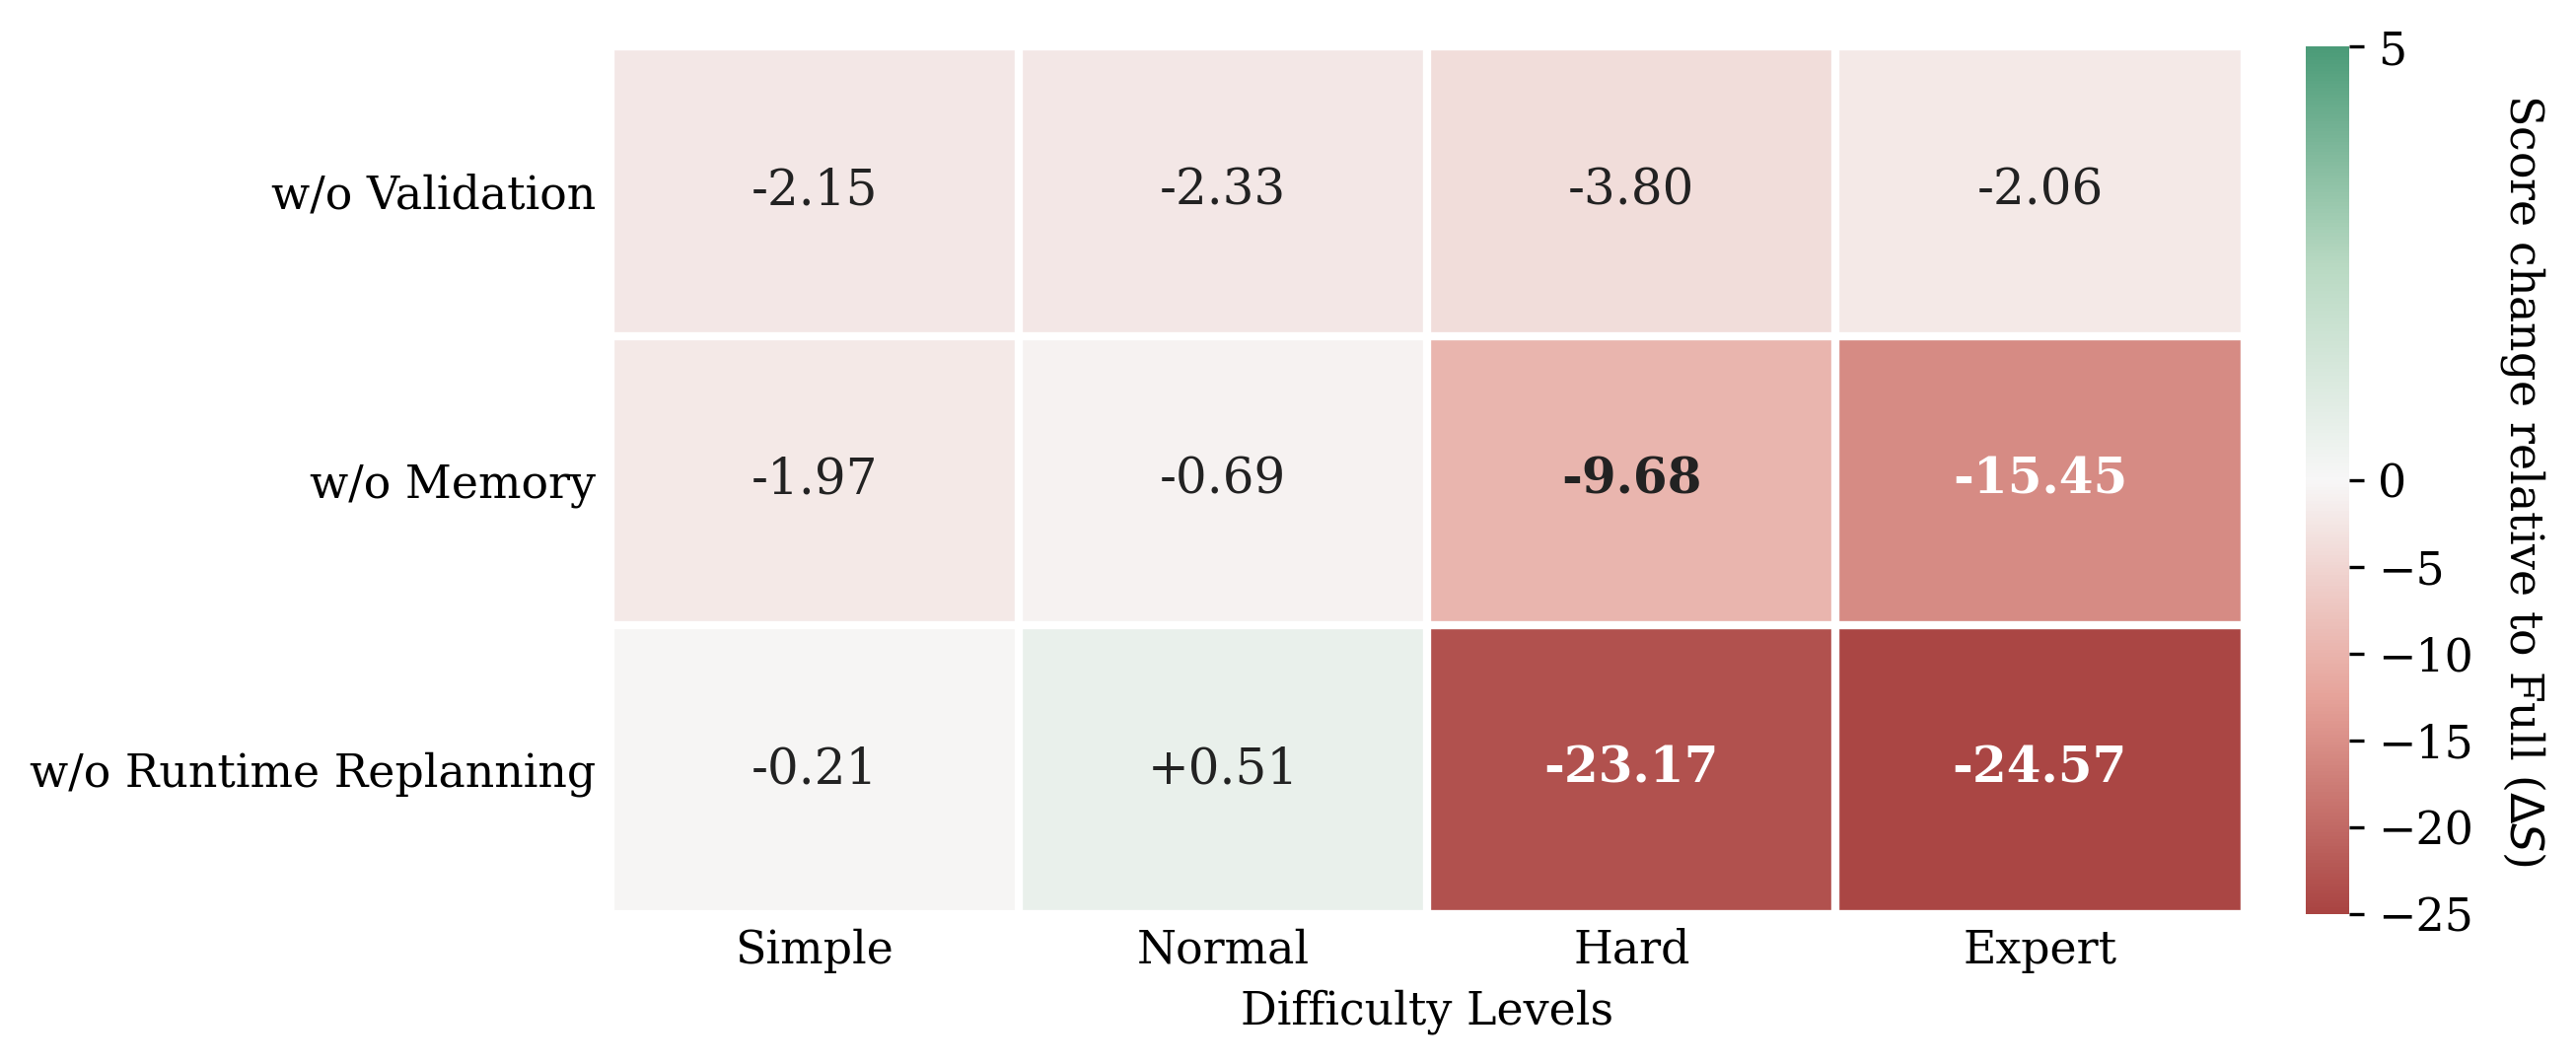
\includegraphics[width=\columnwidth]{figures/ablation-score-change-heatmap.png}
    \caption{Change in overall score relative to CLoMC-UWR for each ablated
    variant and difficulty level. Negative values indicate performance
    degradation, while positive values indicate improvement.}
    \label{fig:ablation-score-delta}
\end{figure}

The contribution of Memory becomes more pronounced as operational pressure
increases.
Removing Memory reduces the score by only 1.97 points in the
simple setting and 0.69 points in the normal setting, but the reduction grows
to 9.68 points in hard episodes and 15.45 points in expert episodes. This
pattern indicates that retrieved task situations, plans, and outcomes are most useful
when resource constraints, event interactions, and scheduling pressure make
planning less routine.

Disabling Runtime Replanning has little effect in the simple and normal
settings, where no perturbations are triggered. In contrast, its score falls
from 59.03 to 35.86 in hard episodes and from 37.55 to 12.98 in expert
episodes. The sharp degradation confirms that an initially valid plan is
insufficient once the execution state changes, and that Runtime Replanning is
the key mechanism for maintaining mission performance under perturbations.

The ablations therefore do not indicate three mechanisms that contribute
uniformly in every episode. Validation acts as a low-frequency safeguard
against invalid candidate plans, Memory contributes most when operational
pressure makes planning less routine, and Runtime Replanning becomes critical
when runtime perturbations invalidate an accepted plan. Their condition-dependent
effects explain why all three are retained in CLoMC-UWR despite
their different average score contributions.

\subsection{Fine-Tuned Planner Evaluation}

\begin{figure}[!t]
    \centering
    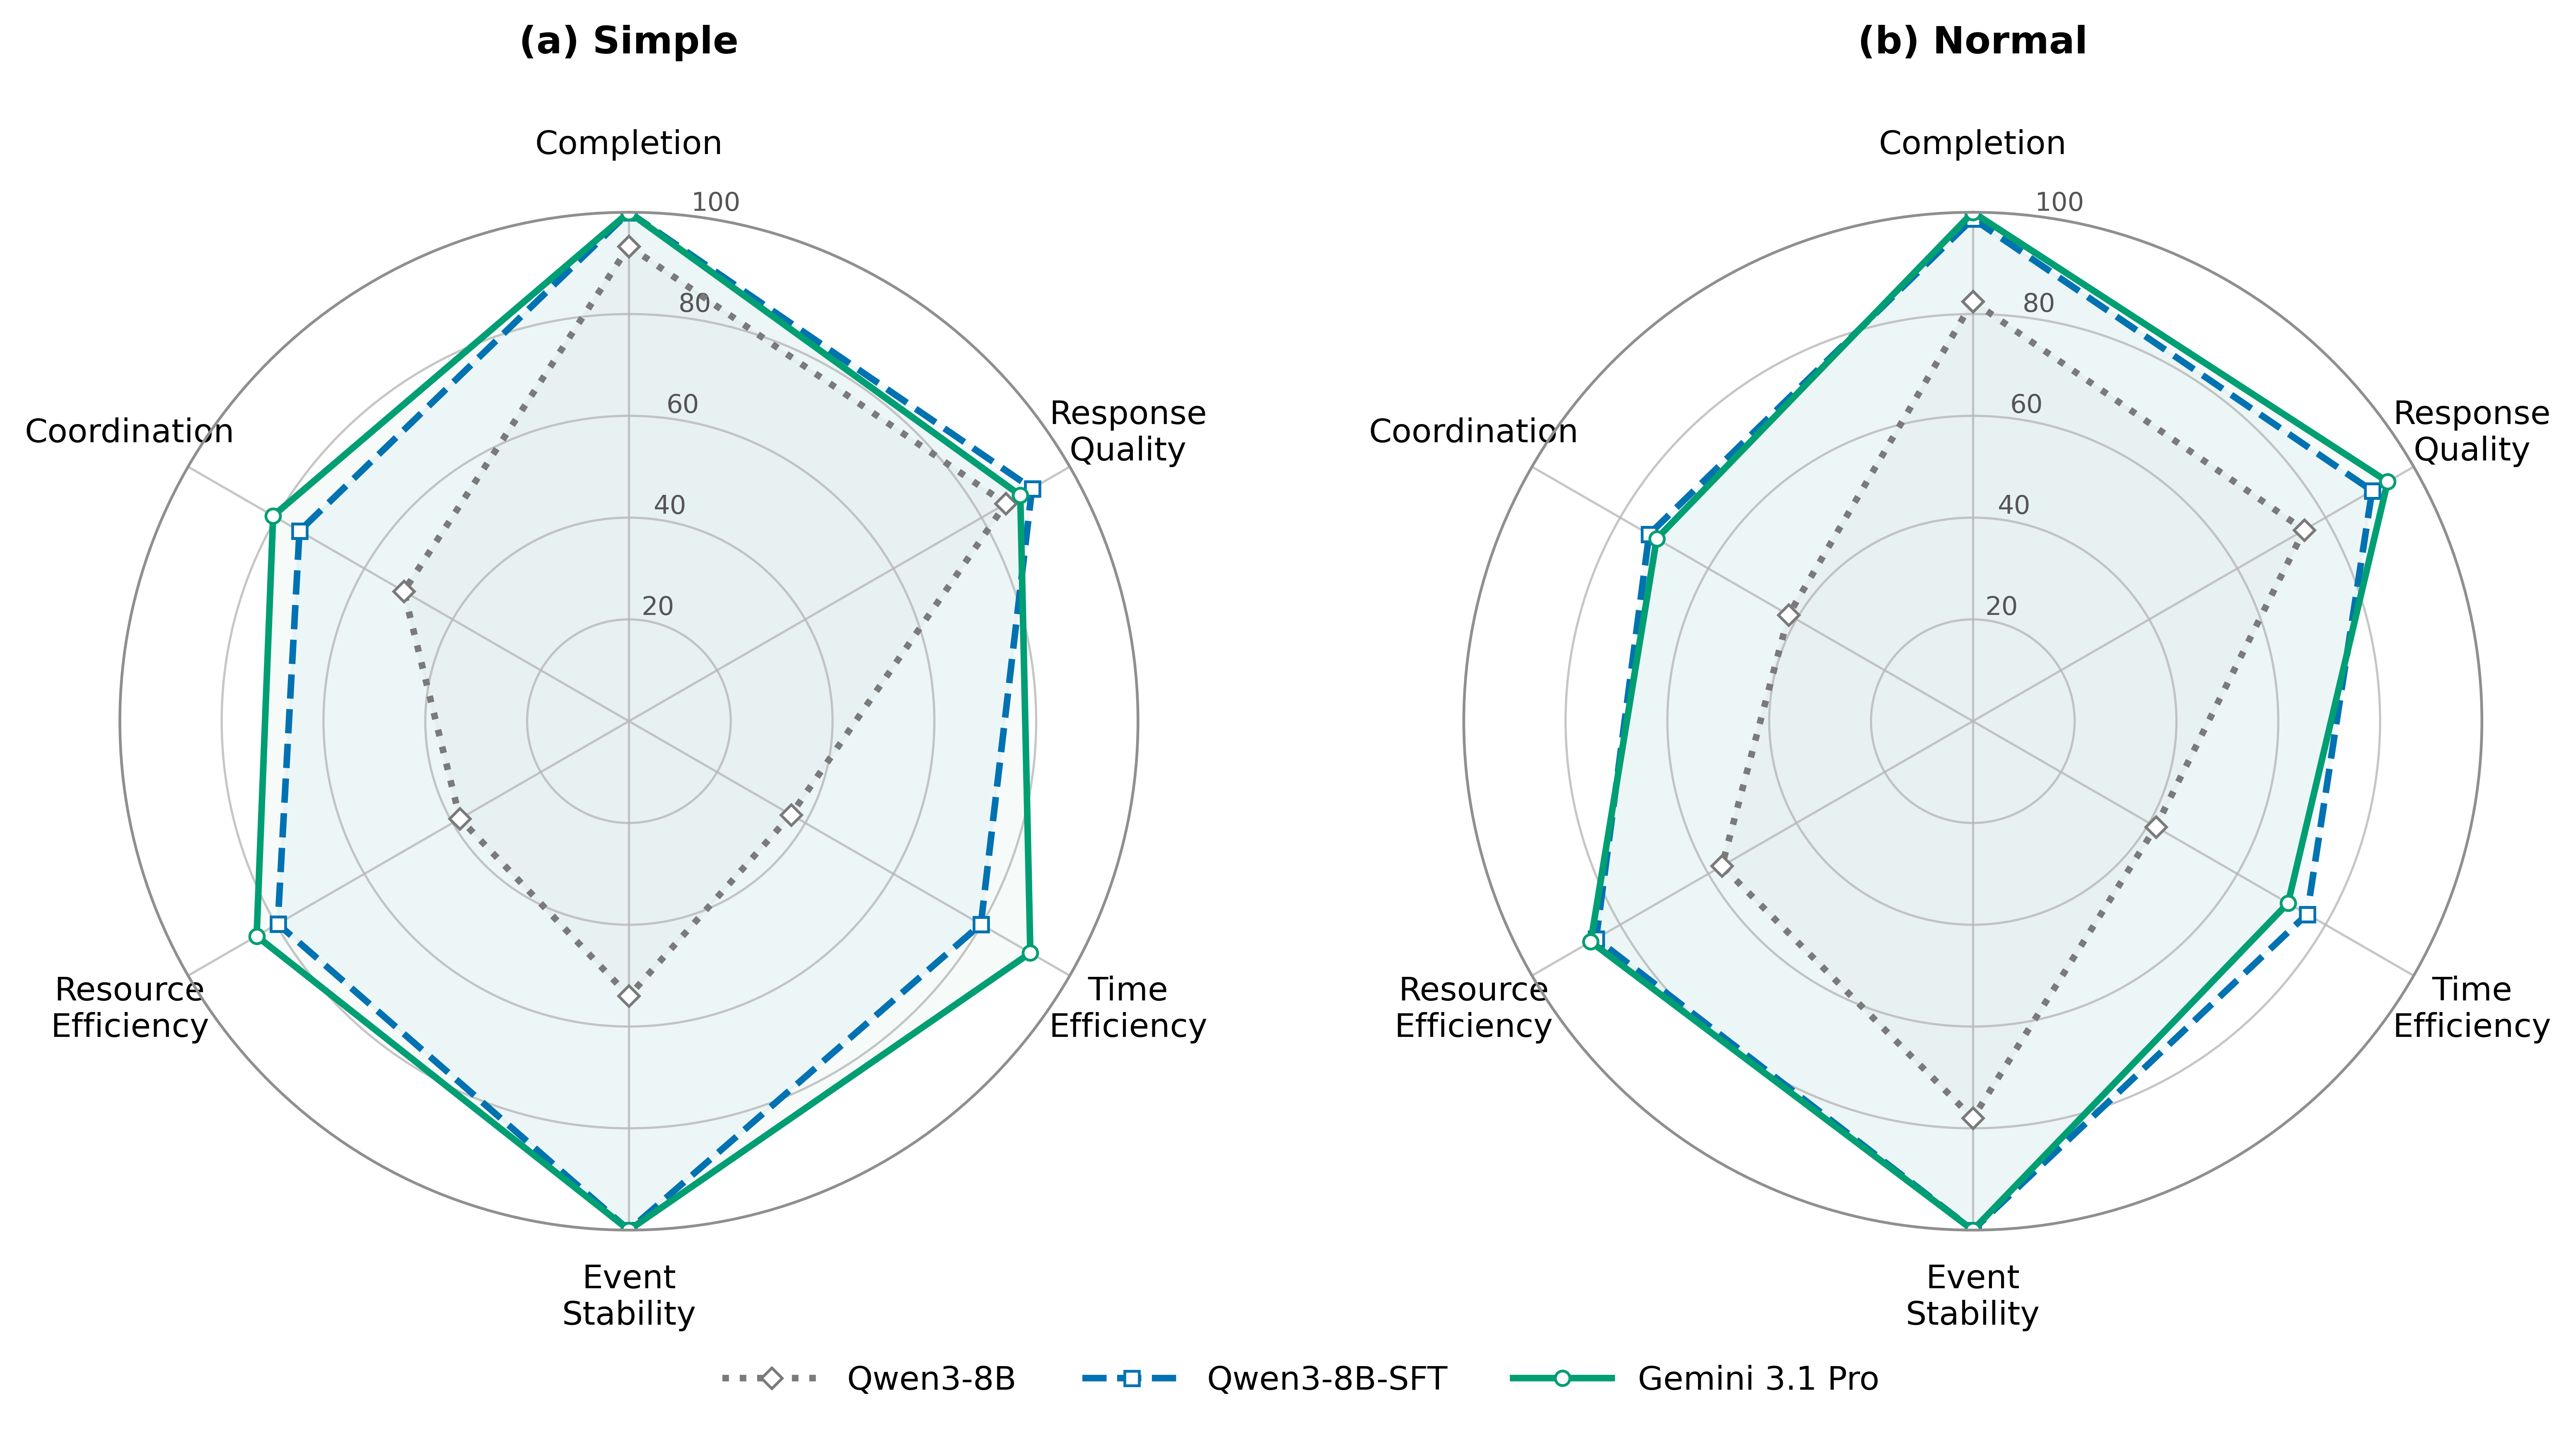
\includegraphics[width=\columnwidth]{figures/planner-performance-radar.png}
    \caption{Mission-level profiles of the three planners in the simple and
    normal settings. Larger radial values indicate better performance. Event
    stability is not interpreted because neither setting contains runtime
    perturbations.}
    \label{fig:planner-performance-radar}
\end{figure}

\begin{figure*}[!b]
    \centering
    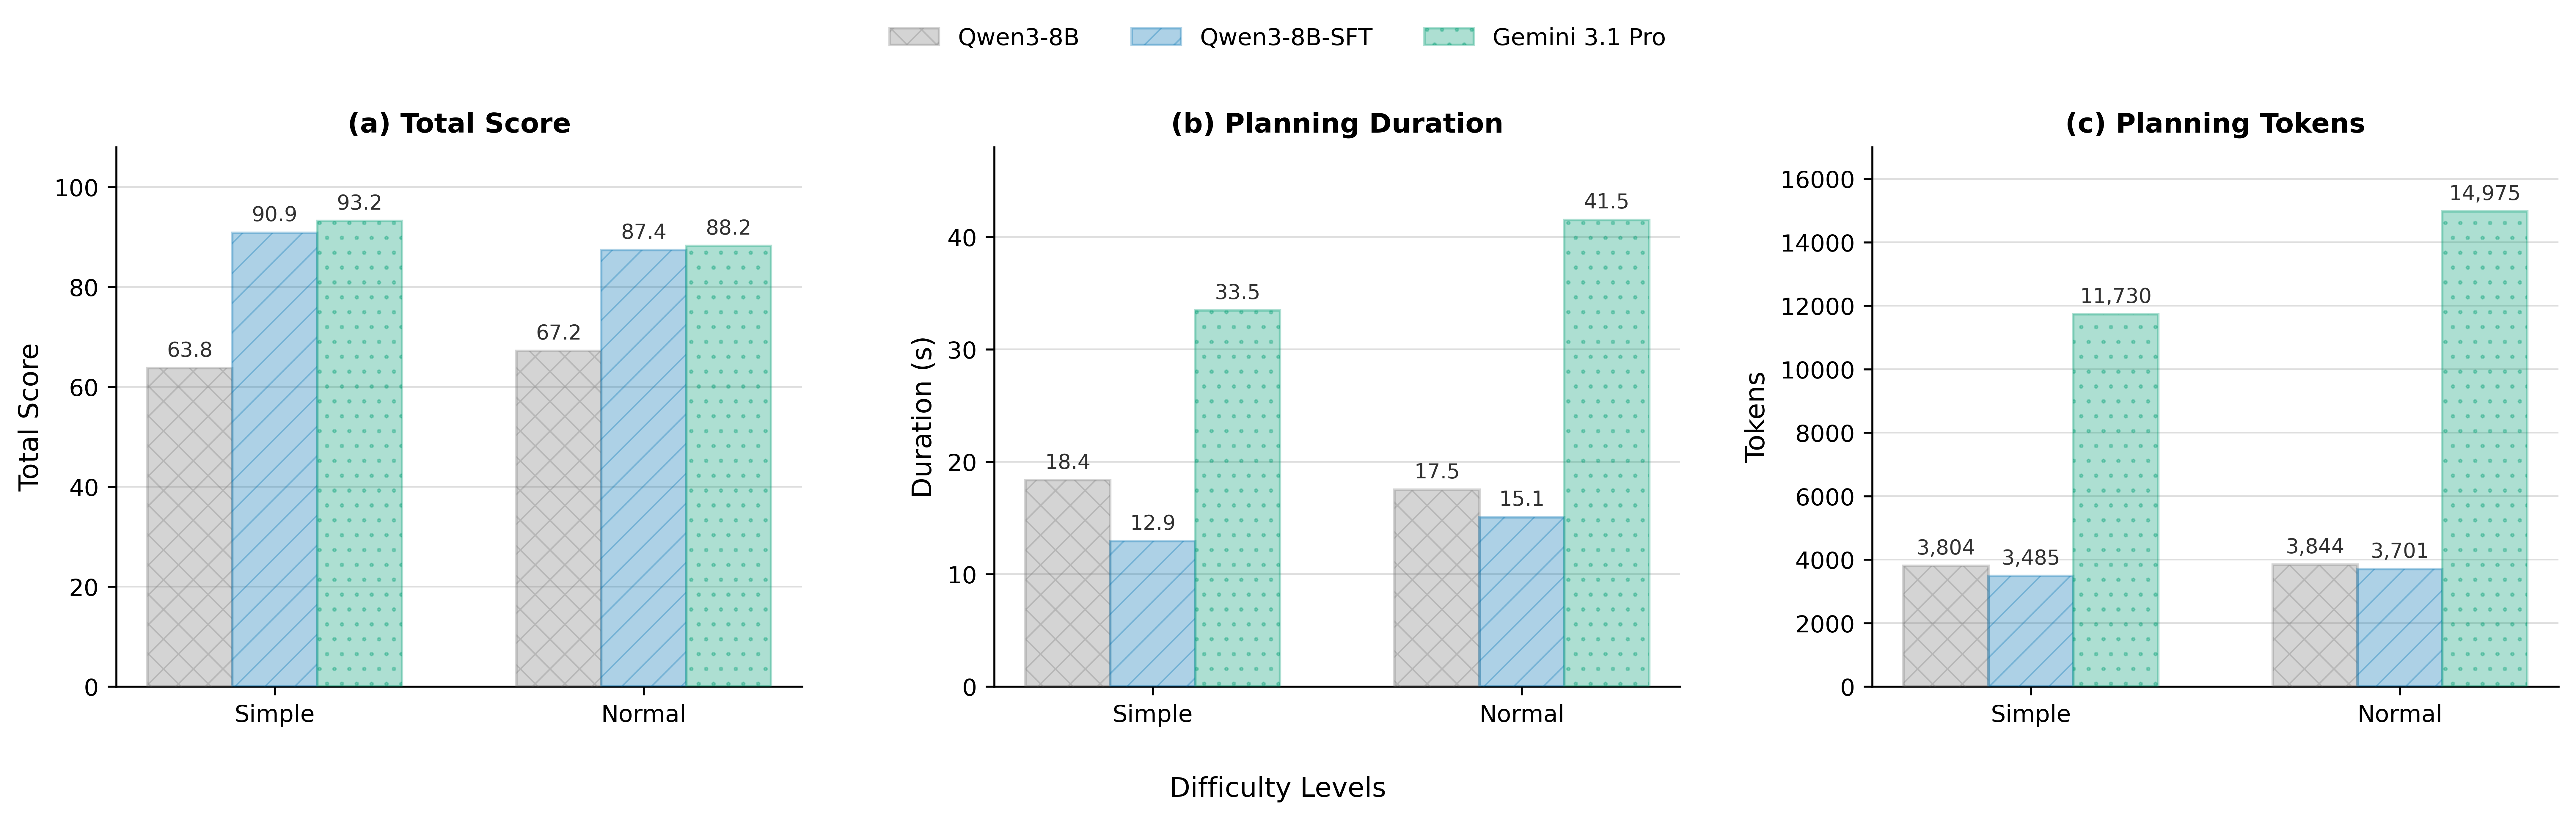
\includegraphics[width=\textwidth]{figures/planner-score-efficiency-comparison.png}
    \caption{Score--efficiency comparison of the three planners: (a) total
    score, (b) planning duration, and (c) planning-token usage. Lower values are
    better in (b) and (c).}
    \label{fig:planner-score-efficiency}
\end{figure*}

Table~\ref{tab:fine-tuned-planner-results} compares the Gemini~3.1~Pro
teacher planner with the original and fine-tuned Qwen3-8B planners. Fine-tuning
substantially improves the compact planner on both difficulty levels, yielding
an average absolute gain of 23.65 points and reaching 98.24\% of the
Gemini~3.1~Pro teacher planner's average score across the simple and normal
settings.

\input{tables/planner-fine-tuning-results}

Figure~\ref{fig:planner-performance-radar} shows that the improvement extends
across the mission-level performance profile. The original Qwen3-8B exhibits
its largest deficits in mission time, resource pressure, and coordination,
whereas fine-tuning substantially expands its profile toward that of
Gemini~3.1~Pro. The fine-tuned planner restores near-complete task coverage and
slightly exceeds Gemini~3.1~Pro in simple-level response and normal-level
mission time and coordination. This indicates that the validated demonstrations
transfer not only output-format compliance but also task-allocation and
resource-management behavior to the compact planner.

The fine-tuned planner also reduces planning overhead under the evaluated
deployment setting. Its mean planning time across the two levels is 14.01~s,
compared with 37.50~s for Gemini~3.1~Pro, while its mean planning-token usage
falls from 13,353 to 3,593. Figure~\ref{fig:planner-score-efficiency} summarizes
this performance--efficiency trade-off. This evidence is limited to initial
planning on the evaluated simple and normal episodes; it does not establish how
the compact planner would perform with Runtime Replanning under hard or expert
conditions.

\FloatBarrier

\endinput
